\documentclass[xcolor=dvipsnames,10pt]{beamer}
\usepackage[utf8]{inputenc}
\usepackage[T1]{fontenc}
\usepackage[brazilian]{babel}
\usepackage{etoolbox}
\usepackage{graphicx}
\usepackage{ragged2e}
\usepackage{tikz}
\usepackage{subfig}
\usepackage{graphics}


\makeatletter
\patchcmd{\beamer@sectionintoc}{\vskip1.5em}{\vskip0.5em}{}{}
\makeatother

\usefonttheme[professional]{serif}

\justifying

%----------------------------------------------------------------------------------------------------------------------------------

% JUSTIFICAR TEXTO DAS LISTAS DE ITENS

\makeatletter
\renewcommand{\itemize}[1][]{%
  \beamer@ifempty{#1}{}{\def\beamer@defaultospec{#1}}%
  \ifnum \@itemdepth >2\relax\@toodeep\else
    \advance\@itemdepth\@ne
    \beamer@computepref\@itemdepth% sets \beameritemnestingprefix
    \usebeamerfont{itemize/enumerate \beameritemnestingprefix body}%
    \usebeamercolor[fg]{itemize/enumerate \beameritemnestingprefix body}%
    \usebeamertemplate{itemize/enumerate \beameritemnestingprefix body begin}%
    \list
      {\usebeamertemplate{itemize \beameritemnestingprefix item}}
      {\def\makelabel##1{%
          {%
            \hss\llap{{%
                \usebeamerfont*{itemize \beameritemnestingprefix item}%
                \usebeamercolor[fg]{itemize \beameritemnestingprefix item}##1}}%
          }%
        }%
      }
  \fi%
  \beamer@cramped%
  \justifying% NEW
  %\raggedright% ORIGINAL
  \beamer@firstlineitemizeunskip%
}
\makeatother

%%%%%%%%%%%%%%%%%%%%%%%%%%%%

%%%%%%%%%%%%%%%%%%%%%%%%%%%%%%%%%%%%%%%%%%%%%%%%%%%%%%%%%%%%%%%%%%%%%%%%%%%%%%%%
%COR DO TEMPLATE SEMELHANTE AO LOGO
%%%%%%%%%%%%%%%%%%%%%%%%%%%%%%%%%%%%%%%%%%%%%%%%%%%%%%%%%%%%%%%%%%%%%%%%%%%%%%%%
\definecolor{azul}{rgb}{0.16, 0.32, 0.75}

%%%%%%%%%%%%%%%%%%%%%%%%%%%%%%%%%%%%%%%%%%%%%%%%%%%%%%%%%%%%%%%%%%%%%%%%%%%%%%%%
%CORES E ESTRUTURAS DE ELEMENTOS DIVERSOS
%%%%%%%%%%%%%%%%%%%%%%%%%%%%%%%%%%%%%%%%%%%%%%%%%%%%%%%%%%%%%%%%%%%%%%%%%%%%%%%%
\setbeamercolor{frametitle}{fg=black}
\setbeamercolor{headline}{fg=black}
\setbeamercolor{footline}{fg=black}
\setbeamercolor{block body}{use=structure,bg=white}
\setbeamercolor{block title}{use=structure,bg=azul,fg=black}
\setbeamercolor{item}{fg=azul}
\setbeamercolor{alerted text}{fg=azul}
\setbeamercolor{section in toc}{fg=black}
\setbeamercolor{title}{fg=black}
\setbeamercolor{subtitle}{fg=black}
\setbeamertemplate{blocks}[rounded][shadow=true]

%%%%%%%%%%%%%%%%%%%%%%%%%%%%%%%%%%%%%%%%%%%%%%%%%%%%%%%%%%%%%%%%%%%%%%%%%%%%%%%%
%PROPRIEDADES VISUAIS DE ELEMENTOS DIVERSOS
%%%%%%%%%%%%%%%%%%%%%%%%%%%%%%%%%%%%%%%%%%%%%%%%%%%%%%%%%%%%%%%%%%%%%%%%%%%%%%%%
\useoutertheme[]{default}
\addtobeamertemplate{block begin}{}{\justifying} % Justify all blocks

\setbeamertemplate{section in toc}[circle]
\setbeamertemplate{subsection in toc}[square]
\setbeamertemplate{itemize item}{$\bullet$}
\setbeamertemplate{navigation symbols}{}
\setbeamercovered{invisible}
\setbeamertemplate{sections in toc}[ball]


%%%%%%%%%%%%%%%%%%%%%%%%%%%%%%%%%%%%%%%%%%%%%%%%%%%%%%%%%%%%%%%%%%%%%%%%%%%%%%%%
%LOGO DO EVENTO COMO TÍTULO DE TODOS OS SLIDES
%%%%%%%%%%%%%%%%%%%%%%%%%%%%%%%%%%%%%%%%%%%%%%%%%%%%%%%%%%%%%%%%%%%%%%%%%%%%%%%%
\setbeamertemplate{headline}{

\vspace{-1em}
\begin{center}

\includegraphics[width=0.7\textwidth]{logo.jpg}
\end{center}
}

%%%%%%%%%%%%%%%%%%%%%%%%%%%%%%%%%%%%%%%%%%%%%%%%%%%%%%%%%%%%%%%%%%%%%%%%%%%%%%%%
% INICIO DOS SLIDES
%%%%%%%%%%%%%%%%%%%%%%%%%%%%%%%%%%%%%%%%%%%%%%%%%%%%%%%%%%%%%%%%%%%%%%%%%%%%%%%%

\title{\textsc{INDICADOR INDIRETO DE ROTAÇÃO EM AGLOMERADOS DE GALÁXIAS}}
\author{
  \textbf{Autor} \\
  Luenne Nailam Sousa Nascimento \\
  \textbf{Orientador} \\
  Prof. Dr. André Luis Batista Ribeiro
}

\begin{document}

\frame{\titlepage}
\frame{\tableofcontents}
\section{Introdução}

\subsection{Aglomerados de Galáxias}

\begin{frame}{\textbf{Aglomerado de Galáxias}}
\begin{itemize}
\item Aglomerados de galáxias são as maiores estruturas do Universo observável que podem ter alcançado o estado em equilíbrio dinâmico.
\item Aglomerados de galáxias são definidos basicamente por três componentes: galáxias, meio intra-aglomerado e matéria escura.
\end{itemize}
 \begin{figure}[!htbp] %h or !htbp
    \begin{center}
    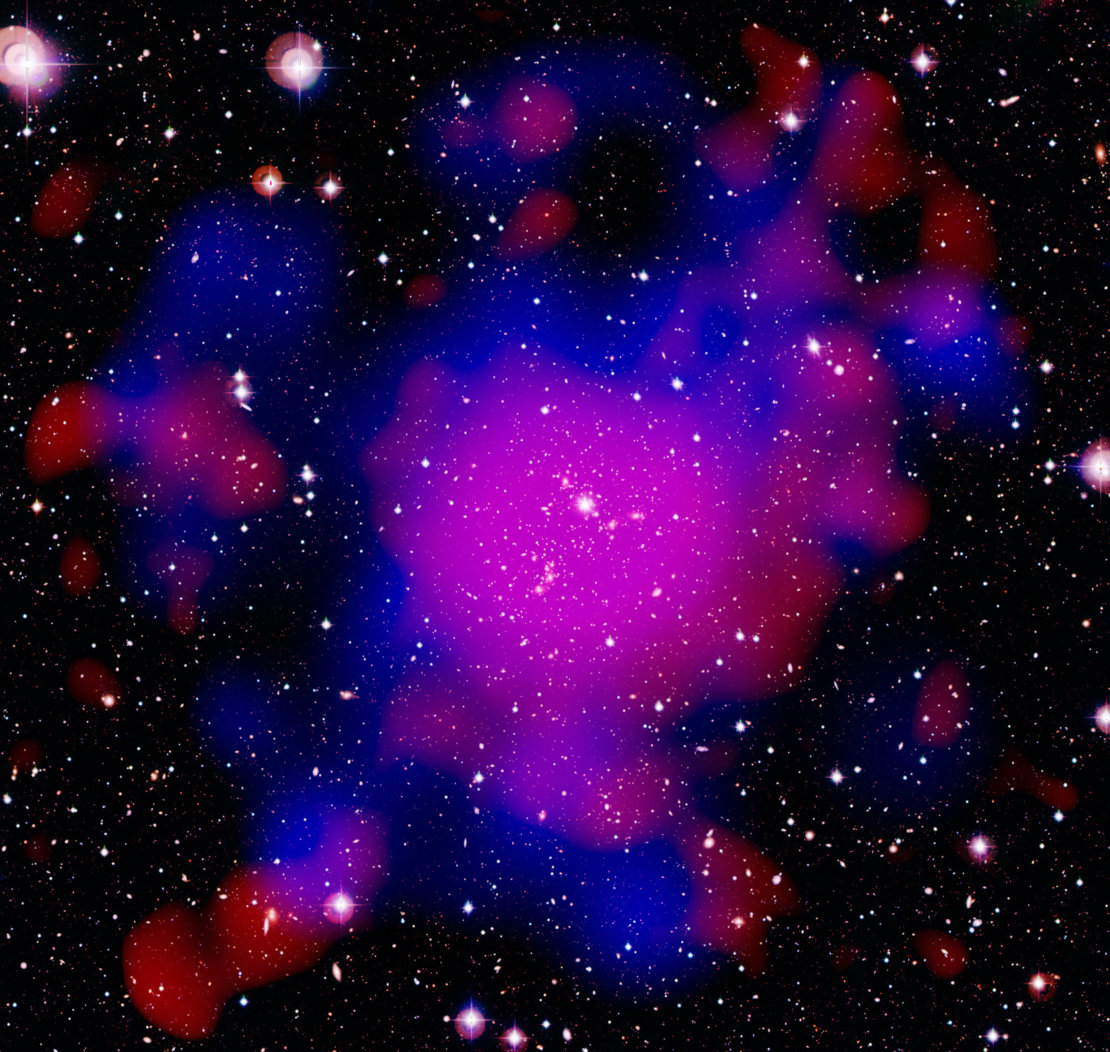
\includegraphics[height=0.5\textheight,width=0.7\textwidth]{resultados/cluster.jpg}%
    \caption{\scriptsize{Composição de um Aglomerado.}}
    \end{center}
  \end{figure} 
\end{frame}

\begin{frame}{\textbf{Aglomerado de Galáxias}}
\begin{itemize}
	\item A busca por compreender a formação e evolução dos aglomerados de galáxias é uma das questões mais importantes da Astrofísica. 
	\item  No paradigma atual de formação das estruturas, as galáxias e os aglomerados surgem a partir de halos escuros.
	\begin{itemize}
	\item Aglomerados formados após as galáxias em um desvio para o vermelho $z \approx 2$.
	\end{itemize}
\end{itemize}
\end{frame}

\begin{frame}{\textbf{Aglomerado de Galáxias}}
 \begin{figure}[!htbp] %h or !htbp
    \begin{center}
    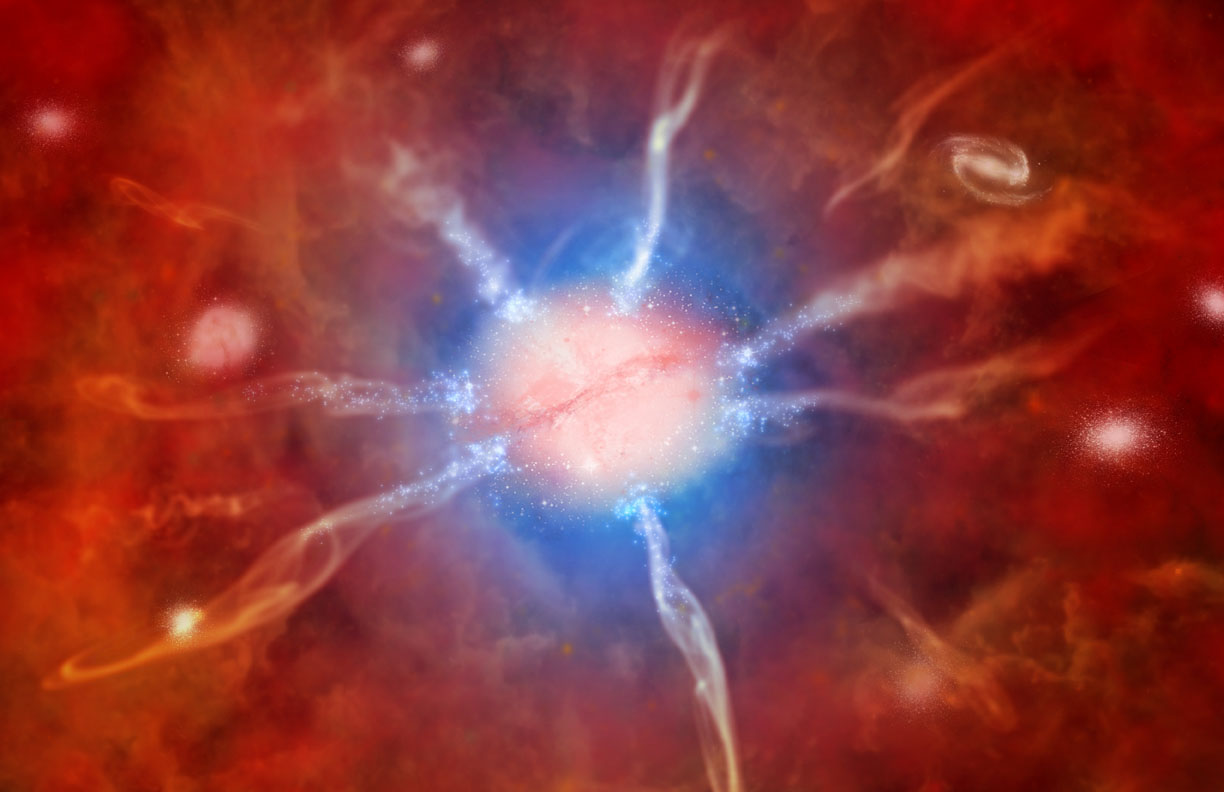
\includegraphics[height=0.5\textheight,width=0.7\textwidth]{resultados/formation.jpg}%
    \caption{\scriptsize{Aglomerado em processo de interação com galáxias ou grupo de galáxias.}}
    \end{center}
  \end{figure} 
\end{frame}

\begin{frame}{\textbf{Aglomerado de Galáxias}}
\begin{itemize}
\item O processo de formação de aglomerados não atingiu seu fim.
\begin{itemize}
\item Distribuição de velocidades é bem ajustada por uma gaussiana somente na região virializada do sistema. Enquanto a periferia do sistema é continuamente perturbada por acréscimo de matéria.
\end{itemize}
\end{itemize}
\end{frame}

\begin{frame}{\textbf{Aglomerado de Galáxias}}
\begin{figure}[!htbp] %h or !htbp
\begin{center}
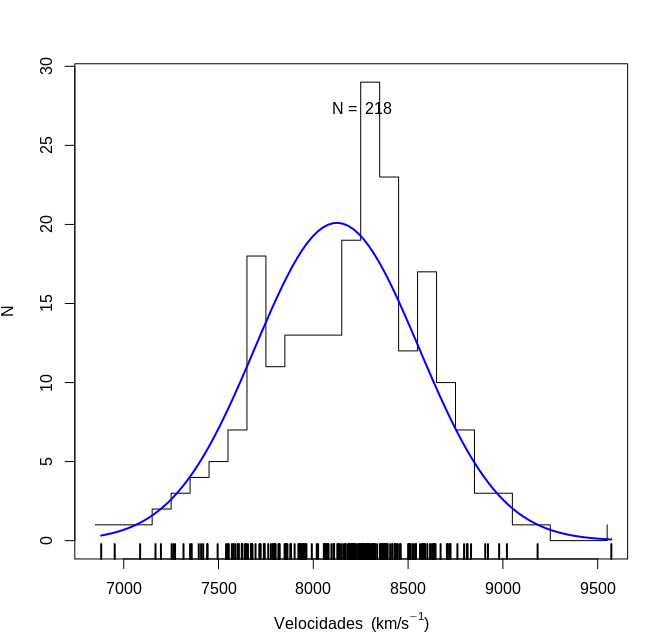
\includegraphics[height=0.6\textheight,width=0.7\textwidth]{10043dist}%
\caption{\scriptsize{Histograma de velocidades de um dos aglomerados de nossa amostra.}}
\label{fig1}%
\end{center}
\end{figure}  
\end{frame}

\subsection{Distribuição de Velocidades ao longo do Aglomerado}
\begin{frame}{\textbf{Distribuição de Velocidades ao longo do Aglomerado}}
\begin{itemize}
\item A velocidade de uma galáxia contida em um aglomerado, em uma dada posição, não pode ser maior que a velocidade de escape do sistema.
\item A velocidade de escape e a distância ao centro do aglomerado são grandezas inversamente proporcionais. 
\item O  perfil radial da velocidade de escape permite definir os galáxias membro dos aglomerados.
\end{itemize} 
\end{frame}

\begin{frame}{\textbf{Distribuição de Velocidades ao longo do Aglomerado}}
  \begin{figure}[!htbp] %h or !htbp
    \begin{center}
    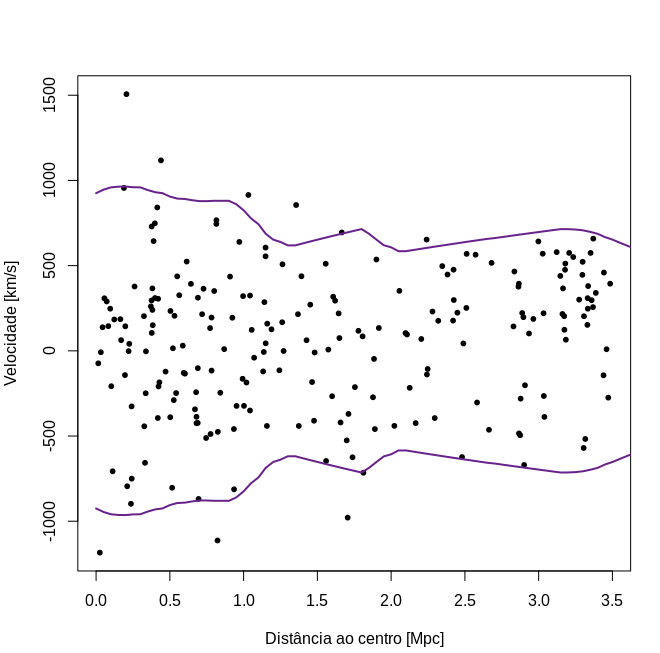
\includegraphics[height=0.6\textheight,width=0.7\textwidth]{10043}%
    \caption{\scriptsize{Distribuição de velocidades em função da distância ao centro de um dos aglomerados de nossa amostra.}}
    \label{fig1}%
    \end{center}
  \end{figure} 
\end{frame}

\begin{frame}
  \begin{itemize}
    \item Após a determinação dos membros de um aglomerado, suas propriedades dinâmicas, como massa e raio, podem ser estimadas.
    \begin{itemize}
      \item O método mais empregado é o de análise do virial.
    \end{itemize} 
  \end{itemize}
  \begin{figure}[!htbp] %h or !htbp
    \begin{center}
    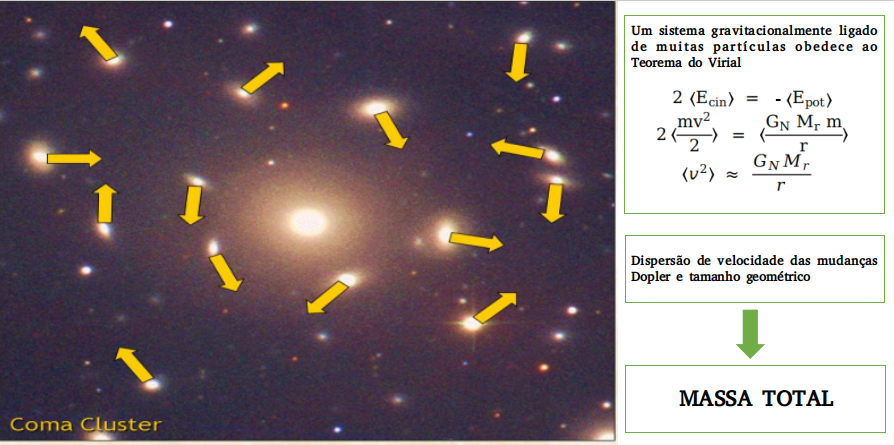
\includegraphics[height=0.5\textheight,width=0.7\textwidth]{resultados/virial.png}%
    \caption{\scriptsize{Análise do virial utiliza apenas as velocidades aleatórias das galáxias na região central do aglomerado.}}
    \end{center}
  \end{figure} 
\end{frame}

\subsection{Rotação de Aglomerados}
\begin{frame}{\textbf{Rotação de Aglomerados}}
\begin{itemize}
  \item {\textbf{Hwang \& Lee (2007):}}  
  \begin{itemize}
    \item \textbf{Amostra:} Dados espectroscópicos do Sloan Digital Sky Survey (SDSS) e Two-Degree-Field Galaxy Redshift Survey (2dF-GRS).
    \item \textbf{Objetivo:} A busca por aglomerados de galáxias que mostrem uma indicação de rotação global.
    \item \textbf{Conclusão e Resultados:}
    \begin{itemize}
      \item Foram detectados seis sistemas com rotação, em um total de doze aglomerados.
      \item Os aglomerados com rotação devem exibir divisão espacial entre galáxias com velocidades maiores e menores que a velocidade média do aglomerado além de apresentar um pico no mapa de densidade.
      \item Constatou-se ainda que estes aglomerados estão em equilíbrio dinâmico e não sofreram fusão recente.
    \end{itemize}
  \end{itemize}
\end{itemize}
\end{frame}

\begin{frame}{\textbf{Rotação de Aglomerados}}
\begin{itemize}
  \item {\textbf{Kalinkov et al. (2008):}}  
    \begin{itemize}
      \item \textbf{Amostra:} Aglomerado de Abell 2107.
      \item \textbf{Objetivo:} Identificar a rotação do aglomerado de galáxias A2107.
      \item \textbf{Conclusão e Resultados:}
      \begin{itemize}
        \item O método buscou o gradiente máximo no campo de velocidade e determinou que a direção do coeficiente de correlação linear máximo definiria o eixo maior do aglomerado e o eixo menor seria o de rotação.
        \item A massa foi corrigida (inicial era de $3.2\times10^{14}~{\rm M_\odot}$ e passou para $2.8\times10^{14}~{\rm M_\odot}$).
        \item Materne et al. (1983) apontaram a dificuldade em diferenciar um aglomerado rotativo de dois que se sobrepõem, pelo motivo de estar se fundindo ou se afastando.
      \end{itemize}
    \end{itemize}
\end{itemize}
\end{frame}

\begin{frame}{\textbf{Rotação de Aglomerados}}
\begin{itemize}
  \item {\textbf{Tovmassian (2015):}}  
    \begin{itemize}
      \item \textbf{Objetivo:} Detectar a rotação de aglomerados de galáxias baseado no estudo da distribuição de velocidades das galáxias membro.
      \item \textbf{Conclusão e Resultados:}
      \begin{itemize}
        \item Constatou-se 17 aglomerados rotativos de 65.
        \item Taxa maior em aglomerados planos $f=a/b > 1.8$, (7 aglomerados rotativos em um total de 18).
        \item Os aglomerados foram originalmente formados a partir das enormes nuvens de gás primordiais e preservaram a rotação das nuvens primordiais, a menos que sofram fusões com outros aglomerados e grupos de galáxias.
      \end{itemize}
    \end{itemize}
\end{itemize}
\end{frame}

\begin{frame}{\textbf{Rotação de Aglomerados}}
\begin{itemize}
  \item {\textbf{Manolopoulou (2014):}}
    \begin{itemize}
      \item \textbf{Amostra:} Inicialmente os testes foram realizados em aglomerados gerados em simulações de Monte Carlo, posteriormente foi utilizado a amostra dos aglomerados de Abell com $z \approx 0.1$ do SDSS DR10.
      \item \textbf{Objetivo:} Identificação de rotação em aglomerados de galáxias usando a velocidade radial projetada.
      \item \textbf{Conclusão e Resultados:}
      \begin{itemize}
        \item Utilizando o teste Kolmogorov-Smirnov, decidiu-se quanto a sua rotação significativa ou não, seu centro rotacional, orientação do eixo de rotação, amplitude de velocidade rotacional e o sentido de rotação no sentido horário ou anti-horário no plano do céu.
        \item Constatou-se 23 aglomerados possivelmente rotativos dentro de 1.5 Mpc ou a uma distância de 2.5 Mpc do centro do aglomerado, de 45 da amostra.
      \end{itemize}
    \end{itemize}
\end{itemize}
\end{frame}

\begin{frame}{\textbf{Rotação de Aglomerados}}
\begin{itemize}
  \item {\textbf{Nascimento et al (2016):}}  
    \begin{itemize}
      \item \textbf{Amostra:} Par de aglomerados de Abell (A3407 e A3408) observadas no Cerro Tololo Interamerican Observatory (CTIO).
      \item \textbf{Objetivo:} Verificar se a amostra correspondia a um simples sistema de galáxias ou a um processo de fusão.
      \item \textbf{Conclusão e Resultados:}
      \begin{itemize}
        \item Ambos os sistemas bem como cada aglomerado individual tem uma distribuição de velocidade Gaussiana.
        \item Um gradiente de velocidade de $\approx 847 \pm 114\; {km/s}$ foi identificada ao redor do eixo principal da distribuição de galáxias projetada.
        \item O estudo do \textit{gap} permitiu encontrar diferença significativa entre estas subamostras.
      \end{itemize}
    \end{itemize}
\end{itemize}
\end{frame}

\section{Objetivos}
\begin{frame}{\textbf{Objetivos}}
  \begin{itemize}
    \item {\textbf{Objetivo Geral: }}
    \begin{itemize}
      \item Detecção da rotação em aglomerados para correção da sua massa.
    \end{itemize}
    \item {\textbf{Objetivos Específicos: }}
    \begin{itemize}
      \item Implementar método de detecção de rotação;
      \item Identificar a velocidade rotacional;
      \item Aplicar o método de Manolopoulou e Plionis (2016) para correção da massa do aglomerado.
    \end{itemize}
  \end{itemize}
\end{frame}

\section{Metologia}

\subsection{Catálogos}
\begin{frame}{\textbf{Catálogo I - selec20}}
  \begin{itemize}
    \item Um catálogo de 20 aglomerados ricos do SDSS, localizados em baixos $redshifts$, com espectroscopia disponível para objetos com $m_r \leq 17.77$.
    \item A amostra foi estudada previamente por Lopes et al. (2009) que definiu e selecionou as galáxias membro estatisticamente.
  \end{itemize}
\end{frame}

\begin{frame}{\textbf{Catálogo II - NoSOCS}}
  \begin{itemize}
    \item Um catálogo de 183 aglomerados, localizados em baixos $redshifts$ ($z \leq 0.10$), elaborado a partir da versão digitalizada do Segundo Levantamento do Observatório de Palomar.
    \item A análise foi estendida para sistemas mais ricos, incluindo os aglomerados CIRS (Cluster Infall Regions in the SDSS) Rines e Diaferio (2006), com 56 objetos.
  \end{itemize}
\end{frame}

\begin{frame}{\textbf{Catálogo III - Simulado}}
  \begin{itemize}
    \item Esferas de NFW (NAVARRO et al., 1997), ou seja, modelos simulados de sistemas esféricos com ou sem rotação
    \item O código foi desenvolvido em linguagem fortran pelo Dr. Claudio Soriano Brandão, cedido para uso neste trabalho.
  \end{itemize}
\end{frame}

\subsection{Algoritmo}
\begin{frame}{\textbf{Algoritmo}}
  \begin{enumerate}
    \item Estudo da distribuição de velocidades das galáxias membro do aglomerado em busca de gaps significativos.
    \begin{itemize}
      \item Identifica a probabilidade de que um \textit{gap}, de certo tamanho e em dada localização, possa ser reproduzido a partir de amostragens aleatórias retiradas de uma gaussiana.
      \item Consideramos \textit{gaps} com valores maiores que 2.25, uma vez que em retiradas aleatórias de uma gaussiana, \textit{gaps} desse tamanho ocorrem no máximo em 3\% dos casos (Wainer \& Shacht 1978. Beers et al. 1991).
    \end{itemize}
  \end{enumerate}
\end{frame}

\begin{frame}{\textbf{Algoritmo}}
  \begin{block}{Valor \textit{gap}}
  \begin{equation}
    g_i = v_{i+1} - v_i
  \end{equation}
  \begin{center}
  \begin{equation}
    w_i=i(N-i)
  \end{equation}
  \begin{center}
  		\hspace{10 ex} exemplo: N = 100\newline
    	\textit{para = 1} \hspace{15 ex}  \textit{para = 50}\newline
    	$w_1 = 1(99) = 99 \hspace{6 ex} w_{50} = 50(50) = 2500$
  \end{center}
  \end{center}
  \begin{equation}
    MM = \frac{2}{N} \sum_{i=N/4}^{3N/4} \sqrt{w_i g_i}
  \end{equation}
  \end{block}
\end{frame}

\begin{frame}{\textbf{Algoritmo}}
  \begin{enumerate}
    \item[2.] Os dados são divididos em duas amostras, contendo objetos com velocidades maiores e velocidades menores do que o maior \textit{gap} (\textbf{Amostras I e II}).
    \item[3.] Determina-se então o eixo principal do aglomerado como aquele resultante do ajuste de uma elipse aos dados projetados no plano do céu (pacote: \textbf{\textit{ellipse}}).
    \item[4.] As amostras I e II são então comparadas em relação a sua distribuição de duas maneiras: independente do eixo principal e em cada lado do eixo.
    \begin{itemize}
      \item Realizamos os testes de Cramér 2D e o de Hotelling.
    \end{itemize}
  \end{enumerate}
\end{frame}

\begin{frame}{\textbf{Algoritmo}}
  \begin{block}{{\textbf{Teste de Crámer 2D}}}
    \begin{itemize}
      \item É uma medida de associação entre duas variáveis nominais dado o intervalo de 0 a 1, indicando que um valor mais alto possui forte associação.
      \begin{equation}
        \ V = \sqrt{\frac{{\chi_{obt}}^2}{N.m}}
        \label{eq:eq1}
        \end{equation}
  
        onde \textbf{$\chi^2$} é o valor obtido do teste estatístico,
        \textbf{N} é o tamanho da amostra e
        \textbf{m} = o menor de (r - 1) ou (c – 1), sendo r o número de linhas e c o número de colunas.
      \item \textbf{Hipótese nula ($H_0$)}: duas amostras não são dependentes uma da outra.
      \item \textbf{Hipótese alternativa ($H_1$)}: existe alguma associação entre duas amostras.
    \end{itemize}
  \end{block}
\end{frame}

\begin{frame}{\textbf{Algoritmo}}
  \begin{block}{{\textbf{Teste de Hotelling}}}
    \begin{itemize}
      \item  Um dos mais conhecidos testes de hipóteses multivariados, o teste de $T^2$, compara vetores de médias populacionais.
      \item Baseado na generalização da estatística \textit{t de Student}, foi o primeiro a levar em consideração a correlação das variáveis na formulação da estatística do teste.
      \begin{equation}
        H_0 : [\mu] = [\mu_0] \hspace{6 ex} H_1 : [\mu] \neq [\mu_0],     
        \end{equation}
  
        onde $[\mu_0]$ é um valor pré-especificado para a forma média.
    \end{itemize}
  \end{block}
\end{frame}

\begin{frame}{\textbf{Algoritmo}}
  \begin{enumerate}
    \item[5.] Dado que as distribuições espaciais das amostras I e II sejam distintas com 95\% de confiança em relação aos testes (passo 4), interpretamos o resultado como sendo uma indicação de rotação nos aglomerados.
    \item[6.] Para os aglomerados onde isto acontece, traçamos um perfil de velocidade de rotação ao longo da distância ao centro do aglomerado.
  \end{enumerate}
\end{frame}

\begin{frame}{\textbf{Fluxograma}}
  \begin{figure}[!htbp]
    \centering
    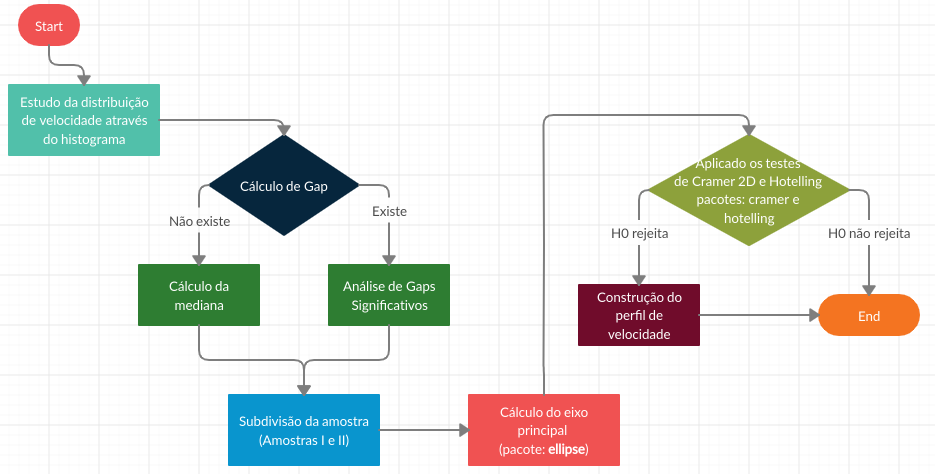
\includegraphics[scale=.3]{resultados/fluxograma.png}
  \end{figure}
\end{frame}

\begin{frame}{\textbf{Método de Hwang \& Lee}}
  \begin{enumerate}
    \item[1.] Método proposto por Hwang e Lee (2007), usualmente aplicado para identificar a rotação em aglomerados.
    \item[2.] Utilizam a relação senoidal para calcular o eixo de rotação ($\Theta_o$) e a velocidade de rotação ($v_{rot}$), através de:

    \begin{equation}
      vp(v_{rot}, \Theta) = v_{sys} + v_{rot} . sin(\Theta - \Theta_o) ,
      \label{eq:hwanglee1}
      \end{equation}
    \item[3.] O procedimento de minimização do $\chi^2$ foi utilizado para determinar o melhor ajuste dos valores de $v_{rot}$ e $\Theta_0$, representado na equação: 
      \begin{equation}
       \chi^2 (v_{rot}, \Theta_o) = \sum_i{\frac{(v_{pi} - v_{los, i})^2}{\sigma^{2}_{i}}} ,
       \label{hwanglee2}
      \end{equation}
  \end{enumerate}
\end{frame}

\begin{frame}{\textbf{Linguagem R}}
	\begin{itemize}
		\item Linguagem que surgiu em 1993 e é considerada multi-paradigma: sequencialização, orientado a objetos, imperativo, dinâmico.
		\item Muito utilizada na manipulação, análise e visualização gráfica de dados.
		\item Pacotes utilizados:
		\begin{itemize}
			\item \textbf{\textit{cramer}};
      \item \textbf{\textit{hotelling}};
      \item \textbf{\textit{nortest}};
      \item \textbf{\textit{ellipse}};
			\item \textbf{\textit{astro}}.
			\item \textbf{\textit{cosmoFns}}.
		\end{itemize}
	\end{itemize}
\end{frame}

\section{Análise}
\begin{frame}{\textbf{Análise}}
  \begin{itemize}
      \item Usamos 1000 réplicas dos dados de velocidade de cada catálogo com intuito de verificar a robustez do método na identificação ou não de rotação.
      \begin{itemize}
        \item \textbf{Catálogo I}: 90\% dos casos (18 aglomerados) obtivemos resultados conclusivos;
        \item \textbf{Catálogo II}: 97.8\% (179 aglomerados) obtivemos resultados conclusivos;
        \item \textbf{Catálogo III}: 100\% dos casos e 97\% (194 aglomerados), para as amostras I e II respectivamente obtivemos resultados conclusivos;
      \end{itemize}
    \end{itemize}
\end{frame}

\begin{frame}{\textbf{Análise}}
  \begin{figure}[!htbp]
    \centering
    \subfloat{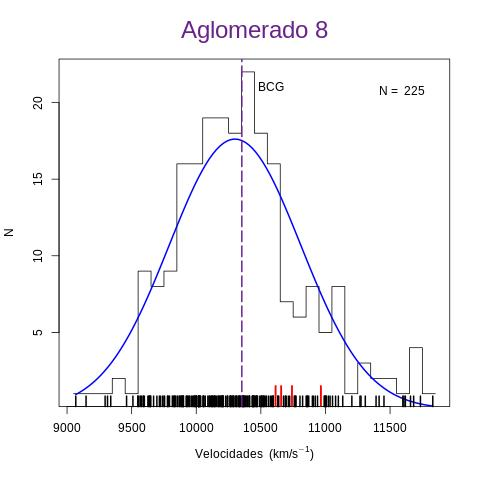
\includegraphics[scale=.28]{resultados/catalogo/selec20gap}}
    \subfloat{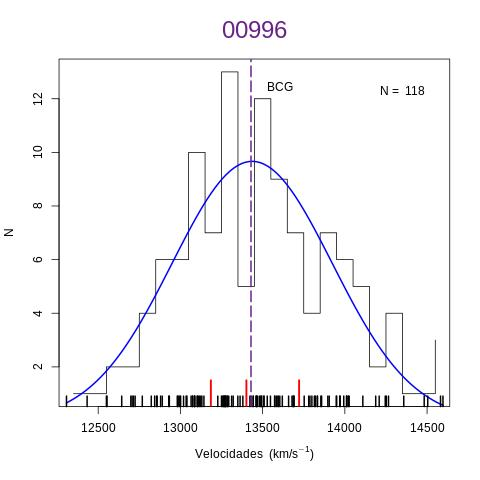
\includegraphics[scale=.28]{resultados/catalogo/dist00996}}
    \caption{Histograma Distribuição de Velocidade e Análise de \textit{gaps} Aglomerados 08 e 00996.}
  \end{figure}
\end{frame}

\begin{frame}{\textbf{Análise}}
  \begin{figure}
     \centering
    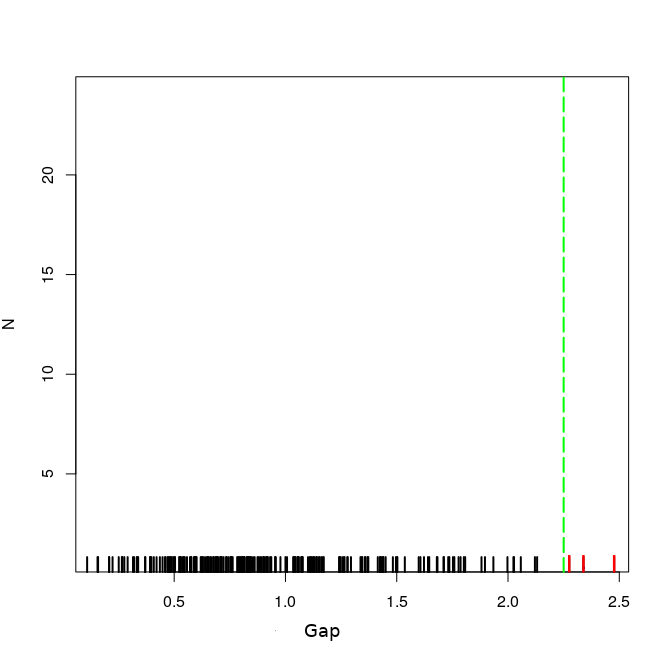
\includegraphics[height=0.7\textheight,width=0.7\textwidth]{resultados/gaps.png}
    \caption{Histograma dos gaps, em vermelho os gaps significativos do Aglomerado 01 e a linha tracejada ao ponto 2.25.}
  \end{figure}
\end{frame}

\begin{frame}{\textbf{Análise}}
  \begin{figure}[!htbp]
    \centering
    \subfloat{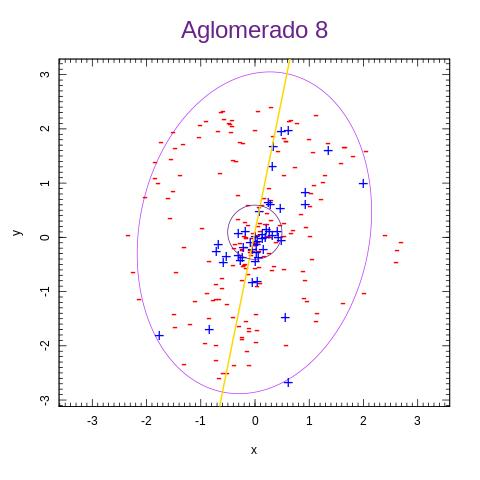
\includegraphics[scale=.28]{resultados/catalogo/selec20ellipse}}
    \subfloat{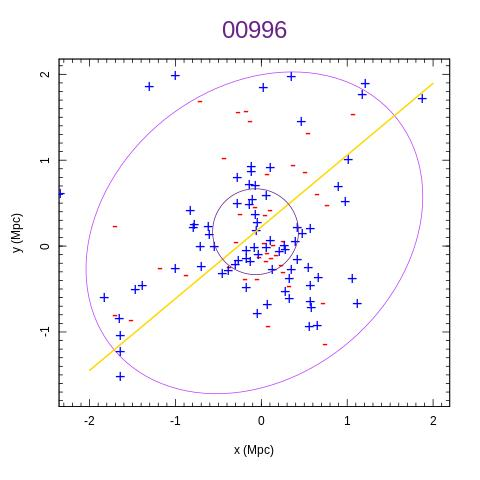
\includegraphics[scale=.28]{resultados/catalogo/eixo00996}}
    \caption{Ajuste da elipse e eixo principal da distribuição projetada no plano do céu aglomerados 08 e 00996.}
  \end{figure}
\end{frame}


\begin{frame}{\textbf{Análise}}
  \begin{table}[H]
  \caption{Teste Cramer e Hotelling aplicado nos aglomerados 08 e 00996.}
  \vspace{12pt}
  \centering{}
  \resizebox{0.85\textwidth}{!}{
  \begin{tabular}{lllllllll}
  \hline
  \multicolumn{1}{c}{\multirow{}{}{\textbf{Cluster}}}     & 
  \multicolumn{2}{|c}{\textbf{Cenário 1}}                     & 
  \multicolumn{2}{c}{\textbf{Cenário 2}}                      & 
  \multicolumn{2}{c|}{\textbf{Cenário 3}}                     & 
  \multicolumn{1}{c}{\multirow{}{}{\textbf{Nº galáxias}}}  \\ \cline{2-7}
  \multicolumn{1}{c}{}                                        & 
  \multicolumn{1}{|c}{\textbf{Cramer}}                        &                 
  \multicolumn{1}{c}{\textbf{Hotelling}}                      & 
  \multicolumn{1}{c}{\textbf{Cramer}}                         & 
  \textbf{Hotelling} & \textbf{Cramer}                        & 
  \multicolumn{1}{l|}{\textbf{Hotelling}}                     & 
  \multicolumn{1}{c}{}                                       & 
  \multicolumn{1}{c}{}                                    
  \\ \hline
  08    &  {\color{red}0.0099} & 0.4446 & {\color{red}0.0119} & 0.0807 & 0.0719 & 0.0551 & 225 \\ 
  00996 & 0.7412 & 0.8761 & 0.5254 & 0.6375 & 0.4935 & 0.8687 & 118 \\ \hline
  \label{tab:selec20T}
  \end{tabular}
  }
  \end{table}
\end{frame}

\begin{frame}{\textbf{Aglomerado com evidência de algum grau de rotação}}
  \begin{itemize}
    \item Aglomerado 08
  \end{itemize}
  \begin{block}{Velocidade de Rotação}
  \begin{equation}
    \omega= \Delta V/R 
  \end{equation}
   \textbf{Unidades:} $V = km/s  \hspace{2 ex} e \hspace{2 ex} R = Mpc$
  \end{block}
\end{frame}


\begin{frame}
  \begin{figure}[!htbp] %h or !htbp
  \vspace{-2pt}
  \begin{center}
  \subfloat{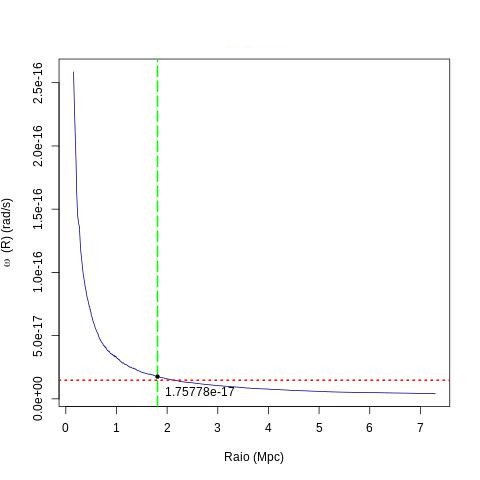
\includegraphics[scale=.3]{resultados/catalogo/rotacao}}
  \caption{Perfil da velocidade de rotação Aglomerado 08.}
  \label{fig6}%
  \end{center}
  \end{figure}
\end{frame}

\begin{frame}
  \begin{block}{{\textbf{Valor limite de detecção de velocidade de rotação}}}
    \begin{itemize}
      \item  Utilizamos a fórmula dada por Lee e Rood (1969) que investigam a dependência da forma e do teorema do virial agindo no movimento orbital.
      \begin{equation}
        \omega \cong \omega_{orb} = \frac{1}{r^2} \sqrt{G M_g \Delta (1 - e^2)}, 
        \label{eq:maxRotacao}
      \end{equation}
  
        \noindent onde $\omega$ é a velocidade de rotação, G é constante gravitacional, R e M são raio e massa do aglomerado, respectivamente, e $e$ é dado por 

        \begin{equation}
        e = 1 - \frac{b}{a}, 
        \label{eq:exce}
\end{equation}

\noindent sendo $a$ e $b$ as distâncias máximas horizontal e vertical ao centro da elipse, respectivamente.
    \end{itemize}
  \end{block}
\end{frame}

\begin{frame}
  \begin{block}{{\textbf{Correção da massa do aglomerado}}}
    \begin{itemize}
      \item  Adotamos a sequência definida por Manolopoulou e Plionis (2016), em que a correção é dada pela diferença relativa entre as dispersões de velocidade do aglomerado corrigida e não-corrigida, sendo definida como
      \begin{equation}
        \delta \sigma_{v} = \frac{\sigma_{v} - \sigma_{v,cor}}{\sigma_{v}},
        \label{eq:corrveldisp}
        \end{equation}

        \noindent e encontramos o valor da massa corrigida utilizando a fórmula abaixo

        \begin{equation}
        M_{cor} \simeq M (1 - \delta \sigma_{v})^2.
        \label{eq:corrmass}
        \end{equation}
    \end{itemize}
  \end{block}
\end{frame}

\begin{frame}
  \begin{block}{{\textbf{Correção da massa do aglomerado}}}
    \begin{itemize}
      \item  Ou podemos realizar o cálculo simplesmente pelo Teorema do Virial dado por:

        \begin{equation}
        M = \frac{v^2 R}{G},
        \label{eq:massa}
        \end{equation}

        \noindent onde $v$ é a velocidade rotacional, $R$ é o raio, $M$ a massa e $G$ é a constante gravitacional.
    \end{itemize}
  \end{block}
\end{frame}

\begin{frame}
  \begin{block}{{\textbf{Correção da massa do aglomerado 08 selec20}}}
    \begin{itemize}
        \item \textbf{$V_{rot}$}: 824.97 $km/s$
        \item M200 : 4.8 $10^{14}  M\odot$ 
        \item \textbf{$M_{cor}$} : 4.04 $10^{14}  M\odot$ 
        \item $\delta \sigma_{v}$ : 0.08
    \end{itemize}
  \end{block}
\end{frame}

\section{Resultados}
\begin{frame}{\textbf{Catálogo I}}
  \\
  {\textbf{Nosso Método}}
  \begin{itemize}
    \item 14.29\% dos aglomerados houve rejeição da hipótese nula (indicando rotação) em pelo menos um dos testes (Cramer e Hotelling) nos três cenários (todos os pontos, acima e abaixo do eixo principal).
    \item 35.71\% dos aglomerados houve rejeição da hipótese nula em pelo menos um dos testes em dois cenários.
    \item 7.14\% dos aglomerados houve rejeição da hipótese nula nos dois testes em apenas um cenário.
  \end{itemize}
\end{frame}

\begin{frame}{\textbf{Catálogo I}}
  \\
  {\textbf{Nosso Método}}
  \begin{itemize}
    \item 7.14\% dos aglomerados houve rejeição da hipótese nula em pelo menos um dos testes em apenas um cenário.
    \item 14.29\% dos aglomerados houve rejeição da hipótese nula em ambos os testes nos três cenários.
    \item 21.42\% dos aglomerados houve rejeição da hipótese nula em ambos os testes em dois cenários.
  \end{itemize}
\end{frame}

\begin{frame}{\textbf{Catálogo I}}
  \\
  {\textbf{Nosso Método}}
  \begin{itemize}
    \item Consideramos evidência significativa de rotação se houve rejeição da hipótese nula em pelo menos um dos cenários testadas.
    \item Isto nos leva a 14 aglomerados com evidência de algum grau de rotação.
    \begin{itemize}
      \item 02, 04, 05, 07, 08, 09, 10, 11, 12, 14, 15, 16, 17 e 18.
    \end{itemize}
  \end{itemize}
\end{frame}

\begin{frame}{\textbf{Catálogo I}}
  \\
  {\textbf{Hwang \& Lee}}
   \begin{table}[H]
      \caption{Resultado do métdo Hwang \& Lee para o catálogo selec20.}
      \vspace{12pt}
      \centering{}
      \resizebox{.5\textwidth}{!}{
      \begin{tabular}{ccccc}
      \cline{1-4}
      \textbf{Cluster} & \textbf{Velocidade Rotacional} & \textbf{Ângulo (radiano)} & \textbf{Ângulo (grau)} \\ \hline
      1 & -724.22 & 2.307 & 132.181 \\
      2 & -661.24 & 2.715 & 155.558 \\
      3 & -1016.65 & 1.767 & 101.242 \\
      4 & 750.69 & 2.092 & 119.863 \\
      5 & -790.08 & 1.197 & 68.583 \\
      6 & 656.37 & 0.785 & 44.977 \\
      7 & -1067.90 & 2.638 & 151.146 \\
      8 & 852.35 & 0.14 & 8.021 \\
      9 & 703.58 & 2.187 & 125.306 \\
      10 & -873.78 & 1.678 & 96.142 \\
      11 & -1117.95 & 2.803 & 160.6 \\
      12 & -946.77 & 3.069 & 175.841 \\
      13 & -891.43 & 2.461 & 141.005 \\
      14 & -625.88 & 0.474 & 27.158 \\
      15 & 864.45 & 0.278 & 15.928 \\
      16 & -1041.45 & 1.011 & 57.926 \\
      17 & -505.15 & 2.556 & 146.448 \\
      18 & 889.73 & 0.812 & 46.524 \\
      19 & -1062.70 & 3.029 & 173.549 \\
      20 & 944.22 & 1.909 & 109.378 \\ \hline
      \end{tabular}
      }
      \label{tab:selec20hwang}
      \end{table}
\end{frame}

\begin{frame}{\textbf{Catálogo I}}
  \begin{figure}[!htbp] %h or !htbp
  \vspace{-2pt}
  \begin{center}
  \subfloat{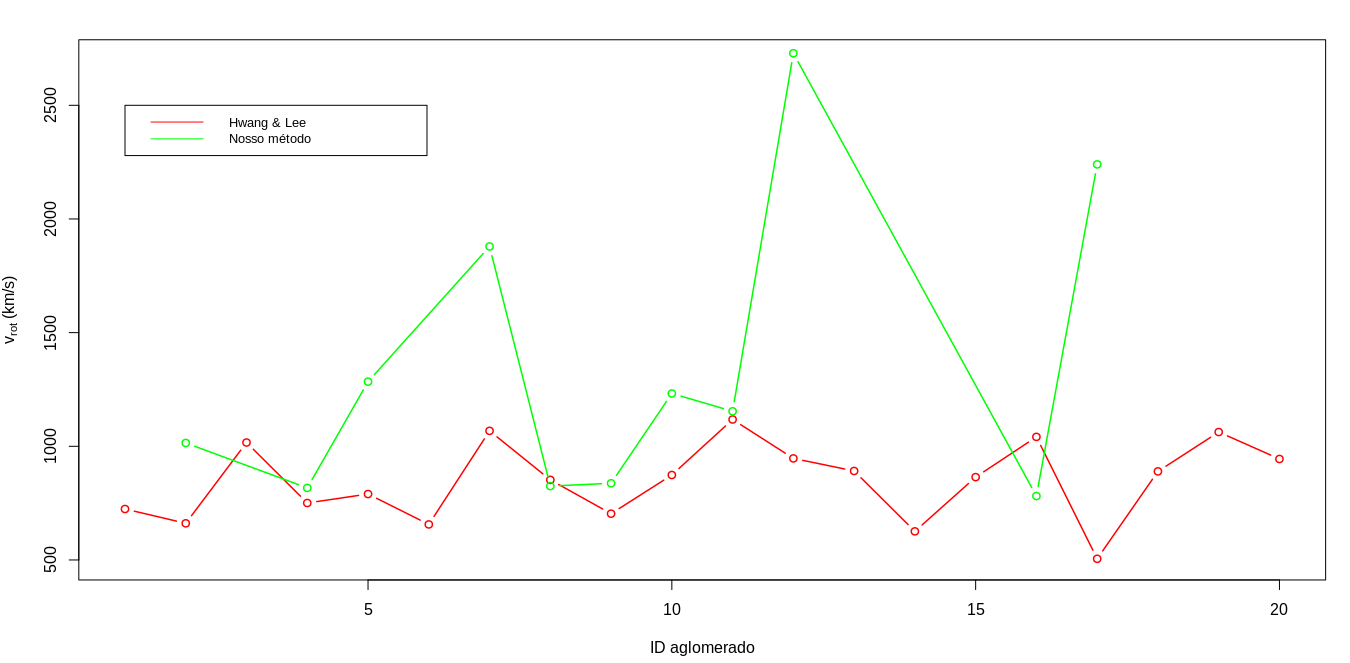
\includegraphics[scale=.20]{resultados/catalogo/selec20vrot}}
  \caption{Comparação das velocidades de rotação encontradas em cada um dos métodos para catálogo selec20.}
  \label{vrotselec20}%
  \end{center}
  \end{figure}
\end{frame}

\begin{frame}{\textbf{Correção da massa}}
  \\
  {\textbf{Catálogo I: Nosso Método}}
  \begin{itemize}
    \item 64\% dos aglomerados (7 dos 11) com indicação de rotação possuem $\delta \sigma$ negativo que implica em um aumento da massa.
    \item 36\% dos aglomerados (4 dos 11) com indicação de rotação possuem $\delta \sigma$ positivo que implica em um redução da massa.
    \item As variações da massa dos aglomerados são significativas, variando de 15.89\% a 28.0\%.
  \end{itemize}
\end{frame}

\begin{frame}{\textbf{Correção da massa}}
  \\
  {\textbf{Catálogo I: Método de Hwang \& Lee}}
  \begin{itemize}
    \item 15\% dos aglomerados (3 dos 20) com indicação de rotação possuem $\delta \sigma$ negativo que implica em um aumento da massa.
    \item 85\% dos aglomerados (17 dos 20) com indicação de rotação possuem $\delta \sigma$ positivo que implica em um redução da massa.
    \item As variações da massa dos aglomerados são significativas, variando de 1.3\% a 52.5\%.
  \end{itemize}
\end{frame}

\begin{frame}{\textbf{Catálogo II}}
  \\
  {\textbf{Nosso Método}}
  \begin{itemize}
    \item Cerca de 25 aglomerados continham um total inferior a 20 objetos, o que tornava o cálculo de detecção de rotação inviável.
    \begin{itemize}
      \item Logo a nossa amostra foi reduzida para 158 aglomerados.
    \end{itemize}
    \item 34.43\% dos aglomerados apresentaram indicação de rotação.
    \item 47.62\% dos sistemas não têm gap, ou seja, em casos onde os dados foram divididos pela mediana.
  \end{itemize}
\end{frame}

\begin{frame}{\textbf{Catálogo II}}
  \\
  {\textbf{Nosso Método}}
  \begin{itemize}
    \item Tendo em conta a rejeição da hipótese em ambos os testes para os três cenários um total de 6.35\%, dois cenários 15.87\% e um cenário 9.52\%.
    \item Já a rejeição da hipótese em pelo menos um dos testes para os três cenários um total de 11.11\%, dois cenários 15.87\% e um cenário 41.27\%.
  \end{itemize}
\end{frame}

\begin{frame}{\textbf{Catálogo II}}
  \\
  {\textbf{Hwang \& Lee}}
  \begin{itemize}
    \item Cerca de 97.26\% dos aglomerados (178) foi detectada rotação. 
    \item Apenas nos aglomerados 02907, 08049, 08720, 09144 e 10046 não identificamos nenhum grau de rotação.
  \end{itemize}
\end{frame}

\begin{frame}{\textbf{Catálogo II}}
  \begin{figure}[!htbp] %h or !htbp
  \vspace{-2pt}
  \begin{center}
  \subfloat{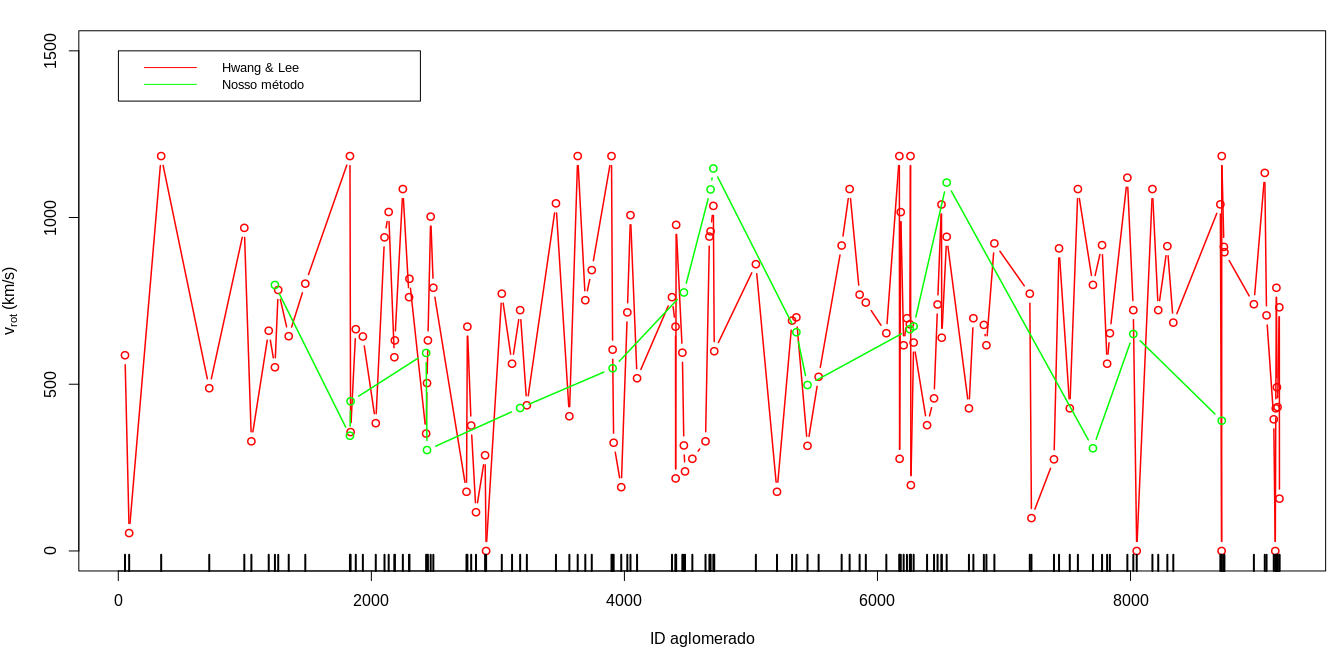
\includegraphics[scale=.20]{resultados/catalogo/nosocsivrot}}
  \caption{Comparação das velocidades de rotação encontradas em cada um dos métodos para catálogo NoSocs.}
  \end{center}
  \end{figure}
\end{frame}

\begin{frame}{\textbf{Catálogo II}}
  \begin{figure}[!htbp] %h or !htbp
  \vspace{-2pt}
  \begin{center}
  \subfloat{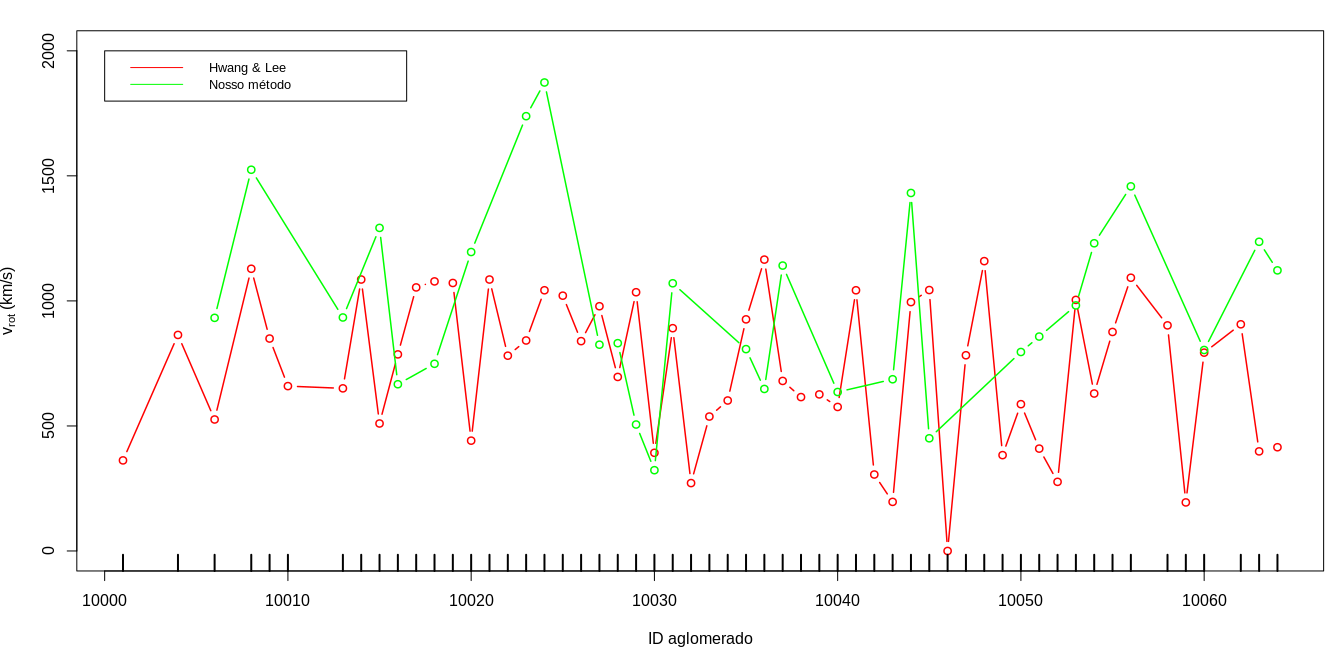
\includegraphics[scale=.20]{resultados/catalogo/nosocsiivrot}}
  \caption{Comparação das velocidades de rotação encontradas em cada um dos métodos para catálogo NoSocs.}
  \end{center}
  \end{figure}
\end{frame}

\begin{frame}{\textbf{Correção da massa}}
  \\
  {\textbf{Catálogo II: Nosso Método}}
  \begin{itemize}
    \item 38.3\% dos aglomerados (18 dos 47) com indicação de rotação possuem $\delta \sigma$ negativo que implica em um aumento da massa.
    \item 59.57\% dos aglomerados (28 dos 47) com indicação de rotação possuem $\delta \sigma$ positivo que implica em um redução da massa.
    \item E em apenas um caso a massa permaneceu inalterada.
    \item As variações da massa dos aglomerados são significativas, variando de 13.48\% a 82.64\%.
  \end{itemize}
\end{frame}


\begin{frame}{\textbf{Correção da massa}}
  \\
  {\textbf{Catálogo II: Método de Hwang \& Lee}}
  \begin{itemize}
    \item 40.45\% dos aglomerados (72 dos 178) com indicação de rotação possuem $\delta \sigma$ negativo que implica em um aumento da massa.
    \item 59.55\% dos aglomerados (106 dos 178) com indicação de rotação possuem $\delta \sigma$ positivo que implica em um redução da massa.
    \item As variações da massa dos aglomerados são significativas, com a taxa superior a 15\%.
  \end{itemize}
\end{frame}

\begin{frame}{\textbf{Catálogo III}}
  \\
  {\textbf{Nosso Método}}
  \begin{itemize}
    \item Geramos duas amostras, com e sem rotação, que chamamos de amostra I e II.
    \item Na amostra I 59.5\% dos casos (119 aglomerados) não apresentaram gaps significativos, portanto utilizamos a mediana.
    \item Já na amostra II o número de casos que não apresentaram gaps significativos foi menor, 18.5\%, ou seja, 37 aglomerados.
  \end{itemize}
\end{frame}

\begin{frame}{\textbf{Catálogo III}}
  \\
  {\textbf{Nosso Método}}
  \begin{itemize}
    \item Amostra I:
    \begin{itemize}
      \item 100\% dos aglomerados apresentaram indicação de rotação.
      \item Desse total, a rejeição da hipótese em ambos os testes para um cenário foi um total de 6\%, dois cenários 5\% e nos três cenários 15\%.
      \item Já a rejeição da hipótese em pelo menos um dos testes para um cenário foi um total de 4\%, dois cenários 11\% e os três cenários 59\%.
    \end{itemize}
  \end{itemize}
\end{frame}

\begin{frame}{\textbf{Catálogo III}}
  \\
  {\textbf{Nosso Método}}
  \begin{itemize}
    \item Amostra II:
    \begin{itemize}
      \item 13.5\% dos aglomerados apresentaram indicação de rotação.
      \item Desse total, a rejeição da hipótese em ambos os testes para um cenário foi um total aproximado de 37.04\%, dois cenários 3.7\%.
      \item Já a rejeição da hipótese em pelo menos um dos testes para um cenário foi um total aproximado de 37.04\%, dois cenários 22.22\%.
    \end{itemize}
  \end{itemize}
\end{frame}

\begin{frame}{\textbf{Catálogo III}}
  \\
  {\textbf{Hwang \& Lee}}
  \begin{itemize}
    \item Na amostra I, em 96.5\% dos casos foi dectectada rotação. O número de falsos negativos (objetos com rotação
que não apresentam indicação para tal) é pequeno, apenas 7 aglomerados teriam este diagnóstico.
    \item Na amostra II, em 97.8\% dos casos houve indicação de algum grau de rotação, quando na verdade nenhum desses sistemas rotaciona. O método de HL é "agressivo"para detectar rotação mas produz uma alta taxa de falsos positivos.
  \end{itemize}
\end{frame}

\begin{frame}{\textbf{Correção da massa}}
  \\
  {\textbf{Catálogo III: Nosso Método}}
  \begin{itemize}
    \item 100\% dos aglomerados com indicação de rotação da amostra I possuem $\delta \sigma$ negativo que implica em um aumento da massa.
    \item Como corresponde a sistemas isolados artificialmente, isto pode indicar que a rotação nestes casos sempre leva a um aumento da massa virial.
  \end{itemize}
\end{frame}

\begin{frame}{\textbf{Correção da massa}}
  \\
  {\textbf{Catálogo III: Método de Hwang \& Lee}}
  \begin{itemize}
    \item 46.12\% dos aglomerados possuem $\delta \sigma$ negativo que implica em um aumento da massa.
    \item 53.88\% dos aglomerados possuem $\delta \sigma$ positivo que implica em uma redução da massa.
  \end{itemize}
\end{frame}

\section{Discussão e Conclusão}
\begin{frame}{\textbf{Comparação entre os métodos}}
  \begin{itemize}
    \item O método de Hwang \& Lee só não detecta rotação nos casos em que a velocidade de rotação é nula ou muita baixa comparando-se a dispersão de velocidades do aglomerado.
    \begin{itemize}
      \item Na amostra simulada o método detectou excessivos aglomerados com rotação. 
    \end{itemize}
    \item O nosso método permite que o usuário defina o seu grau de conservadorismo frente aos resultados, levando em conta os testes estatísticos.
    \item Ou seja, de modo geral, nosso método detectará um menor número de aglomerados com rotação do que HL, mas os nossos resultados são mais robustos. 
  \end{itemize}
\end{frame}

\begin{frame}{\textbf{Comparação entre os métodos}}
  \begin{itemize}
    \item Nosso método obtém em poucos casos valores mais altos das velocidades de rotação. Se removidos, podemos notar um razoável acordo para as velocidades obtidas, considerando-se que são métodos aproximativos e com alto grau de incertezas devido à falta de informação tridimensional.     
    \item O aumento ou a diminuição da massa depende do fator de correção $\delta \sigma$ ser negativo ou positivo. Isto acontece nas amostras observadas, enquanto na amostra simulada os resultados dos métodos divergem.
      \begin{itemize}
        \item Esta diferença de resultados é um ponto a ser investigado futuramente.
      \end{itemize}
  \end{itemize}
\end{frame}

\begin{frame}{\textbf{Comparação entre os métodos}}
  \begin{itemize}
    \item Não é conclusiva a relação entre a normalidade da distribuição de velocidades e a ocorrência de rotação.   
    \begin{itemize}
      \item No catálogo selec20 parece haver um forte favorecimento da correlação rotação-não-gaussianidade.
        \begin{itemize}
          \item 81.82\% rejeitaram a $H_0$, aplicado o método de Anderson Darling.
        \end{itemize}
      \item No catálogo NoSOCS isto não acontece.
        \begin{itemize}
            \item 44.68\% rejeitaram a $H_0$, aplicado o método de Anderson Darling.
          \end{itemize}
    \end{itemize}
  \end{itemize}
\end{frame}

\section{Perspectivas}
\begin{frame}{\textbf{Perspectivas}}
  \begin{itemize}
    \item Implementar e testar o método de Manolopoulou e Plionis (2016).
    \item Fazer uma seleção de aglomerados com indicação de rotação acima de 1000 $km/s$ para buscar contrapartida em dados em raios-X.
    \item Definir um erro estatístico em torno das velocidades de rotação encontradas.
    \item Refazer a comparação dos métodos, já levando em conta o de Manolopoulou e Plionis (2016), usando um catálogo mais extenso, compreendendo pelo menos 500 aglomerados.
  \end{itemize}
\end{frame}

\begin{frame}{\textbf{Perspectivas}}
  \begin{itemize}
    \item Compreender a significativa diferença de resultados para a correção de massa de sistemas simulados, esferas de NFW, entre o nosso método e HL.
    \item Nos casos em que os sistemas estiverem fora do equilíbrio, obter uma nova expressão para a massa corrigida.
  \end{itemize}
\end{frame}

\section{Referências}
\begin{frame}{Referências}
  \begin{thebibliography}{9}
  \fontsize{8}{0}\selectfont
    \bibitem [ANDREON et~al, 2012]{ANDREON2012} 
      ANDREON, Stefano; BERGÉ, J. Richness-mass relation self-calibration for galaxy clusters. Astronomy \& Astrophysics, v. 547, p. A117, 2012.

    \bibitem [BACHMAN et~al, 2017]{BACHMAN2017}
      BACHMAN, Ronet; PATERNOSTER, Raymond. Statistics for criminology and criminal justice. SAGE, 2017.

    \bibitem [BEERS et~al, 1991]{BEERS1991}
      BEERS, Timothy C. et al. A dynamical analysis of twelve clusters of galaxies. The Astronomical Journal, v. 102, p. 1581-1609, 1991.

    \bibitem [BULLOCK et~al, 2001]{BULLOCK2001}
      BULLOCK, James S. et al. Profiles of dark haloes: evolution, scatter and environment. Monthly Notices of the Royal Astronomical Society, v. 321, n. 3, p. 559-575, 2001.

    \bibitem [CIRILLO et~al, 2003]{CIRILLO2003}
      CIRILLO, Marcelo Angelo; FERREIRA, Daniel Furtado. Extensão do teste para normalidade univariado baseado no coeficiente de correlação quantil-quantil para o caso multivariado. Revista de Matemática e Estatística, São Paulo, v. 21, n. 3, p. 67-84, 2003.

  \end{thebibliography}
\end{frame}

\begin{frame}{Referências}
  \begin{thebibliography}{9}
  \fontsize{8}{0}\selectfont
  \bibitem [COMERFORD et~al, 2007]{COMERFORD2007}
  COMERFORD, Julia M.; NATARAJAN, Priyamvada. The observed concentration–mass relation for galaxy clusters. Monthly Notices of the Royal Astronomical Society, v. 379, n. 1, p. 190-200, 2007.

  \bibitem [COMPUTING et~al, 2019]{COMPUTING2019}
  COMPUTING, Statistical. Disponível em:< http://www. R-project. org/>. Acesso em, v. 10, 2012. de agosto de 2019.

  \bibitem [CRAMER et~al, 2004]{CRAMER2004}
  CRAMER, Duncan; HOWITT, Dennis Laurence. The Sage dictionary of statistics: a practical resource for students in the social sciences. Sage, 2004.

  \bibitem [DUPKE et~al, 2006]{DUPKE2006}
  DUPKE, Renato A.; BREGMAN, Joel N. Direct measurements of gas bulk flows in the intracluster medium of the centaurus cluster with the Chandra satellite. The Astrophysical Journal, v. 639, n. 2, p. 781, 2006.

  \bibitem [FANG et~al, 2009]{FANG2009}
  FANG, Taotao; HUMPHREY, Philip; BUOTE, David. Rotation and turbulence of the hot intracluster medium in galaxy clusters. The Astrophysical Journal, v. 691, n. 2, p. 1648, 2009.
  \end{thebibliography}
\end{frame}

\begin{frame}{Referências}
  \begin{thebibliography}{9}
  \fontsize{8}{0}\selectfont
  \bibitem [FRIACA et~al, 2000]{FRIACA2000}
  FRIAÇA, Amâncio César Santos et al. Astronomia: uma visão geral do universo. 2000.

  \bibitem [GAL et~al, 2003]{GAL2003}
  GAL, R. R. et al. The northern sky optical cluster survey. II. An objective cluster catalog for 5800 square degrees. The Astronomical Journal, v. 125, n. 4, p. 2064, 2003.

  \bibitem [GAL et~al, 2004]{GAL2004}
  GAL, R. R. et al. The Northern Sky Optical Cluster Survey. I. Detection of Galaxy Clusters in DPOSS. The Astronomical Journal, v. 119, n. 1, p. 12, 2000.

  \bibitem [GAL et~al, 2009]{GAL2009}
  GAL, R. R. et al. The northern sky optical cluster survey. iii. a cluster catalog covering pi steradians. The Astronomical Journal, v. 137, n. 2, p. 2981, 2009.

  \bibitem [GALI et~al, 2003]{GALI2004}
  GAL, Roy R. et al. The digitized second palomar observatory sky survey (DPOSS). II. Photometric calibration. The Astronomical Journal, v. 128, n. 6, p. 3082, 2004.
  \end{thebibliography}
\end{frame}

\begin{frame}{Referências}
  \begin{thebibliography}{9}
  \fontsize{8}{0}\selectfont
  \bibitem [HWANG et~al, 2007]{HWANG2007}
  HWANG, Ho Seong; LEE, Myung Gyoon. Searching for rotating galaxy clusters in SDSS and 2dFGRS. The Astrophysical Journal, v. 662, n. 1, p. 236, 2007.

  \bibitem [KALINKOV et~al, 2005]{KALINKOV2005}
  KALINKOV, M. et al. Rotation of the cluster of galaxies A2107. Monthly Notices of the Royal Astronomical Society, v. 359, n. 4, p. 1491-1497, 2005.

  \bibitem [LEE et~al, 1969]{LEE1969}
  LEE, See-Woo; ROOD, Hervert L. The Shape and Virial Theorem of a Star Cluster in the Galactic Tidal Force Field. Journal of Korean Astronomical Society, v. 2, p. 1-9, 1969.

  \bibitem [LEOTTI et~al, 2012]{LEOTTI2012}
  LEOTTI, Vanessa Bielefeldt; COSTER, Rodrigo; RIBOLDI, João. Normalidade de variáveis: métodos de verificação e comparação de alguns testes não-paramétricos por simulação. Revista HCPA. Porto Alegre. Vol. 32, no. 2 (2012), p. 227-234, 2012.

  \bibitem [LIEBER et~al, 1990]{LIEBER1990}
  LIEBER, Richard L. Statistical significance and statistical power in hypothesis testing. Journal of Orthopaedic Research, v. 8, n. 2, p. 304-309, 1990.
  \end{thebibliography}
\end{frame}

\begin{frame}{Referências}
  \begin{thebibliography}{9}
  \fontsize{8}{0}\selectfont
  \bibitem [LIU et~al, 2019]{LIU2019}
  LIU, Ang; TOZZI, Paolo. Testing the rotation versus merger scenario in the galaxy cluster Abell 2107. Monthly Notices of the Royal Astronomical Society, v. 485, n. 3, p. 3909-3918, 2019.

  \bibitem [LOPES et~al, 2009]{LOPE2009}
  LOPES, P. A. A. et al. NoSOCS in SDSS–I. Sample definition and comparison of mass estimates. Monthly Notices of the Royal Astronomical Society, v. 392, n. 1, p. 135-152, 2009.

  \bibitem [LOPES et~al, 2006]{LOPE2006}
  LOPES, Paulo AA et al. X-ray Galaxy Clusters in NoSOCS: Substructure and the Correlation of Optical and X-ray Properties. The Astrophysical Journal, v. 648, n. 1, p. 209, 2006.

  \bibitem [LOPES et~al, 2004]{LOPE2004}
  LOPES, Paulo AA et al. The northern sky optical cluster survey. iv. an intermediate-redshift galaxy cluster catalog and the comparison of two detection algorithms. The Astronomical Journal, v. 128, n. 3, p. 1017, 2004.

  \bibitem [MANOLOPOULOU et~al, 2016]{MANOLOPOULOU2016}
  MANOLOPOULOU, Maria; PLIONIS, Manolis. Galaxy cluster's rotation. Monthly Notices of the Royal Astronomical Society, p. stw2870, 2016.
  \end{thebibliography}
\end{frame}

\begin{frame}{Referências}
  \begin{thebibliography}{9}
  \fontsize{8}{0}\selectfont
  \bibitem [MATERNE et~al, 1983]{MATERNE1983}
  MATERNE, J.; HOPP, U. The cluster of galaxies SC0316-44-Does it rotate?. Astronomy and Astrophysics, v. 124, p. L13-L15, 1983.

  \bibitem [MUDHOLKAR et~al, 2000]{MUDHOLKAR2000}
  MUDHOLKAR, Govind S.; SRIVASTAVA, Deo Kumar. Robust analogs of Hotelling's two-sample T2. Communications in Statistics-Theory and Methods, v. 29, n. 12, p. 2717-2749, 2000.

  \bibitem [NASCIMENTO et~al, 2016]{NASCIMENTO2016}
  NASCIMENTO, R. S. et al. Dynamical analysis of the cluster pair: A3407+ A3408. Monthly Notices of the Royal Astronomical Society, v. 460, n. 2, p. 2193-2206, 2016.

  \bibitem [NASCIMENTO et~al, 2012]{NASCIMENTO2012}
  NASCIMENTO, R. S. Estudo da dinâmica de pares de aglomerados de galáxias. Dissertação (Mestrado) — Universidade Estadual de Santa Cruz, Ilhéus, 2012.

  \bibitem [NAVARRO et~al, 1997]{NAVARRO1997}
  NAVARRO, Julio F.; FRENK, Carlos S.; WHITE, Simon DM. A universal density profile from hierarchical clustering. The Astrophysical Journal, v. 490, n. 2, p. 493, 1997.
  \end{thebibliography}
\end{frame}

\begin{frame}{Referências}
  \begin{thebibliography}{9}
  \fontsize{8}{0}\selectfont
  \bibitem [OEGERLE et~al, 1992]{OEGERLE1992}
  OEGERLE, William R.; HILL, John M. Structure, rotation, and the peculiar velocity cD galaxy in Abell 2107. The Astronomical Journal, v. 104, p. 2078-2085, 1992.

  \bibitem [OLIVEIRA et~al, 2004]{OLIVEIRA2004}
  OLIVEIRA F.; VIEGAS, S. M. M. de. Astronomia: Uma Visão Geral do Universo. [S.l.]: EDUSP, 2004.

  \bibitem [REMBOLD et~al, 2011]{REMBOLD2011}
  REMBOLD, S. B. Tópicos especiais em física: Astronomia. Ilhéus: Editora Editus, 2011.

  \bibitem [RIBEIRO et~al, 2011]{RIBEIRO2011}
  RIBEIRO, A. L.; LOPES, P. A.; TREVISAN, M. Non-gaussian velocity distributions—the effect on virial mass estimates of galaxy groups. Monthly Notices of the Royal Astronomical Society: Letters, Blackwell Science Ltd Oxford, UK, v. 413, n. 1, p. L81–L85, 2011.

  \bibitem [RINES et~al, 2006]{RINES2006}
  RINES, K.; DIAFERIO, A. Cirs: Cluster infall regions in the sloan digital sky survey. i. infall patterns and mass profiles. The Astronomical Journal, IOP Publishing, v. 132,n. 3, p. 1275, 2006.
  \end{thebibliography}
\end{frame}

\begin{frame}{Referências}
  \begin{thebibliography}{9}
  \fontsize{8}{0}\selectfont
  \bibitem [RYDEN et~al, 2017]{RYDEN2017}
  RYDEN, B. Introduction to cosmology. [S.l.]: Cambridge University Press, 2017.

  \bibitem [SAMPAIO et~al, 2013]{SAMPAIO2013}
  SAMPAIO, F. S. Estudo da Distribuição de velocidades em aglomerados de galáxias - Testes de Não Rejeitaidade e metanálise de Fisher. Dissertação (Mestrado) — Universidade Estadual de Santa Cruz, Ilhéus, 2013.

  \bibitem [SONG et~al, 2018]{SONG2018}
  SONG, H.; HWANG, H. S.; PARK, C.; SMITH, R.; EINASTO, M. A redshift survey of the nearby galaxy cluster a2107: Global rotation of the cluster and its connection to large-scale structures in the universe. The Astrophysical Journal, IOP Publishing, v. 869, n. 2, p. 124, 2018.

  \bibitem [SPRINGEL et~al, 1999]{SPRINGEL1999}
  SPRINGEL, V.; WHITE, S. D. Tidal tails in cold dark matter cosmologies. Monthly Notices of the Royal Astronomical Society, Wiley Online Library, v. 307, n. 1, p. 162–178, 1999.

  \bibitem [TOVMASSIAN et~al, 2015]{TOVMASSIAN2015}
  TOVMASSIAN, H. M. The rotation of galaxy clusters. Astrophysics, Springer, v. 58, n. 3, p. 328–337, 2015.
  \end{thebibliography}
\end{frame}

\begin{frame}{Referências}
  \begin{thebibliography}{9}
  \fontsize{8}{0}\selectfont
  \bibitem [VELÁSQUEZ et~al, 2007]{VELÁSQUEZ2007}
  VELÁSQUEZ, C. A. M. Estimativa de Parâmetros Cosmológicos usando Aglomerados de Galáxias. Dissertação (Mestrado) — Universidade Federal do Rio de Janeiro, Rio de Janeiro, 2007.

  \bibitem [WAINER et~al, 1978]{CWAINER1978}
  WAINER, H.; SCHACHT, S. Gapping. Psychometrika, Springer, v. 43, n. 2, p. 203–212, 1978.

  \bibitem [YAHIL et~al, 1977]{YAHIL1977}
  YAHIL, A.; VIDAL, N. The velocity distribution of galaxies in clusters. The Astrophysical Journal, v. 214, p. 347–350, 1977.
  \end{thebibliography}
\end{frame}

\end{document}
